% 08_feature_importance_floats.tex -- tables and figures for this section (2026-10-15), each \input from a generated/ file or an
% \includegraphics of a generated figure; generators: writeup/make_rehaul_*.py. Placed after the section in paper_rehaul.tex
% so section text and floats can be edited in parallel; move them inline when the prose settles.
%
% DRAFT floats (the section is still a skeleton): every caption opens "Draft, measures under review". Caption numbers
% are \rhapp... macros from generated/rehaul_app_numbers.tex (writeup/make_rehaul_appendix.py). Figures:
%   results/feature_importance_1530_dedup/fig_ranked_all_features.png, fig_rank_heatmap_all_features_{series,cluster}.png
%     -- RASTER: regenerate as PDF (drawn by experiments/feature_importance_1530.py's aggregate stage);
%   figures/feature_importance_1530_over_time{,_linear}.pdf -- vector (writeup/feature_importance_1530_dedup_sections.py).
% Table: generated/rehaul_app_featimp_harma.tex, a re-layout of generated/appendix_campaign_16h_featimp.tex (which
% overflows the text width at \small).
\ifdefined\rhappNdays\else% AUTO-GENERATED by writeup/make_rehaul_appendix.py -- do not edit.
% Source: every number quoted in rehaul/10_appendix_floats.tex and rehaul/08_feature_importance_floats.tex captions
\newcommand{\rhappNdays}{866}
\newcommand{\rhappNblocks}{5}
\newcommand{\rhappAllbarsRinitAll}{0.2298}
\newcommand{\rhappAllbarsRinitBase}{0.2358}
\newcommand{\rhappAllbarsWdBAll}{0.2630}
\newcommand{\rhappAllbarsWdBBase}{0.2480}
\newcommand{\rhappNvariants}{35}
\newcommand{\rhappNmonthEnd}{43}
\newcommand{\rhappNextreme}{60}
\newcommand{\rhappNother}{763}
\newcommand{\rhappNmonthEndExtreme}{5}
\newcommand{\rhappExtremeCols}{10}
\newcommand{\rhappGapShareExtreme}{71}
\newcommand{\rhappGapShareMonthEnd}{60}
\newcommand{\rhappGapShareOther}{\ensuremath{-}31}
\newcommand{\rhappNcolsBase}{22}
\newcommand{\rhappNcolsAll}{628}
\newcommand{\rhappNsessionEdge}{12}
\newcommand{\rhappNsessionEdgeHalf}{6}
\newcommand{\rhappOptExch}{20}
\newcommand{\rhappOptTrials}{50}
\newcommand{\rhappOptPoints}{1{,}469}
\newcommand{\rhappShiftNfc}{9}
\newcommand{\rhappShiftNdays}{865}
\newcommand{\rhappShiftKmin}{\ensuremath{-}12}
\newcommand{\rhappShiftKmax}{6}
\newcommand{\rhappShiftNnot}{85}
\newcommand{\rhappMurphyNc}{33}
\newcommand{\rhappModelSetN}{94}
\newcommand{\rhappModelSetPaper}{9}
\newcommand{\rhappModelSetPooledLin}{6}
\newcommand{\rhappModelSetPerBarLin}{7}
\newcommand{\rhappModelSetPerBarTrees}{72}
\newcommand{\rhappCompF}{3}
\newcommand{\rhappCompDays}{614}
\newcommand{\rhappFiRefits}{147}
\newcommand{\rhappFiSeries}{49}
\newcommand{\rhappFiClusters}{166}
\newcommand{\rhappFiColsEligible}{564}
\newcommand{\rhappFiBootBlock}{6}
\newcommand{\rhappFiDraws}{10}
\newcommand{\rhappFiClusterCorr}{0.8}
\newcommand{\rhappFiRefitEvery}{10}
\newcommand{\rhappFiTimeTop}{5}
\newcommand{\rhappFiTimeSmooth}{5}
\newcommand{\rhappFiTimeCap}{20}
\newcommand{\rhappFiConstCols}{137}
\fi

% Source: results/feature_importance_1530_dedup/fig_ranked_all_features.png (raster)
% 2026-10-15 (user): parked -- non-standard figure; focus on legible tables
% \begin{figure}[htbp]
% \centering
% 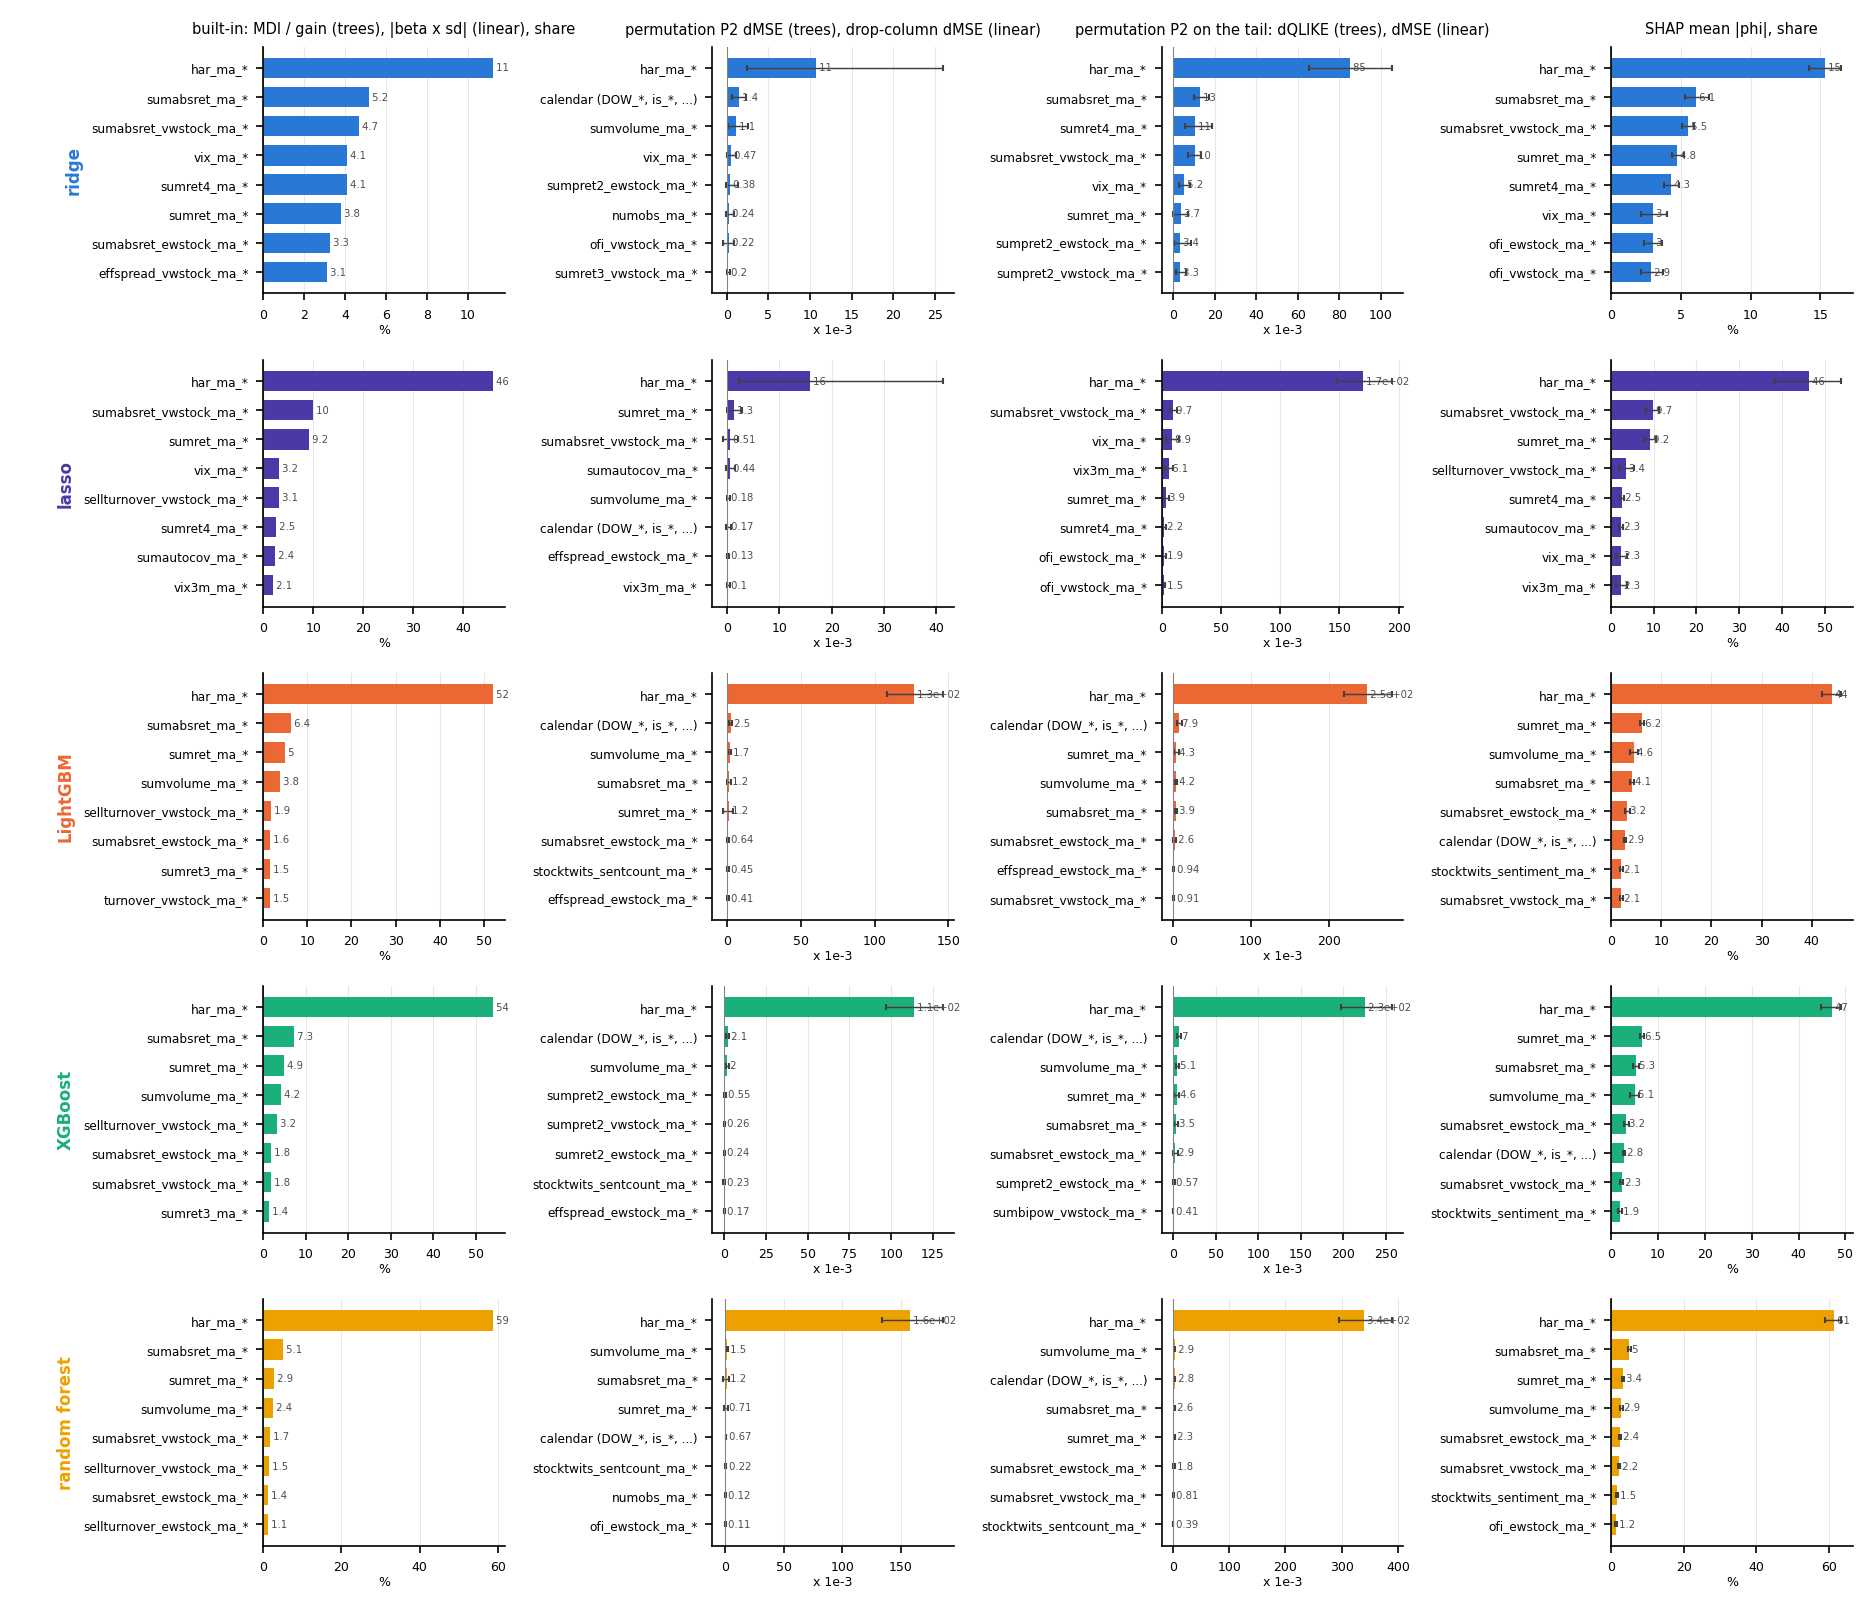
\includegraphics[width=\linewidth]{../results/feature_importance_1530_dedup/fig_ranked_all_features.png}
% % 2026-10-15 (notation pass): parked -- code jargon (refits, P2, fit space, held-out tail, |beta . sd|); standard measure names
% % \caption{Draft, measures under review. The leading series by each measure, per model (rows), all features
% % (\rhappNcolsAll{} columns in \rhappFiSeries{} series), averaged over the \rhappFiRefits{} refits. Columns: the
% % built-in measure (MDI\,/\,gain share for the trees, $|\beta\cdot\mathrm{sd}|$ share for the linear models);
% % permutation P2, $\Delta$MSE in the fit space (trees), or drop-column $\Delta$MSE (linear); permutation P2 on the
% % held-out tail, $\Delta$QLIKE (trees) or $\Delta$MSE (linear); SHAP mean $|\phi|$ share. Whiskers: 95\,\%
% % circular-block bootstrap intervals over refits (block \rhappFiBootBlock), which the paper's point-estimate convention
% % would drop.}
% \caption{Draft, measures under review. Leading predictor series by importance measure, for each closing-interval
% model (rows), on the full predictor set (\rhappNcolsAll{} columns in \rhappFiSeries{} series), averaged over the
% \rhappFiRefits{} re-estimations. Columns: the model's built-in measure (share of mean decrease in impurity, MDI, or of
% gain for the trees; share of $|\beta_j|\,\mathrm{sd}(x_j)$ for the linear models); permutation importance, the
% increase in squared-error loss on the scale of the target $y_t$ (trees), or the drop-column increase in squared-error
% loss (linear models); permutation importance on the out-of-sample block, the increase in QLIKE (trees) or in
% squared-error loss (linear models); and the share of the mean absolute SHAP value $|\phi|$. Permutation importance
% replaces a predictor's values with rows drawn from the estimation window. Whiskers: 95\% circular block-bootstrap
% confidence intervals across re-estimations (block length \rhappFiBootBlock); elsewhere the paper reports point
% estimates.}
% \label{fig:rh_app_fi_ranked}
% \end{figure}

% Source: results/feature_importance_1530_dedup/fig_rank_heatmap_all_features_series.png (raster)
% 2026-10-15 (user): parked -- non-standard figure; focus on legible tables
% \begin{figure}[htbp]
% \centering
% 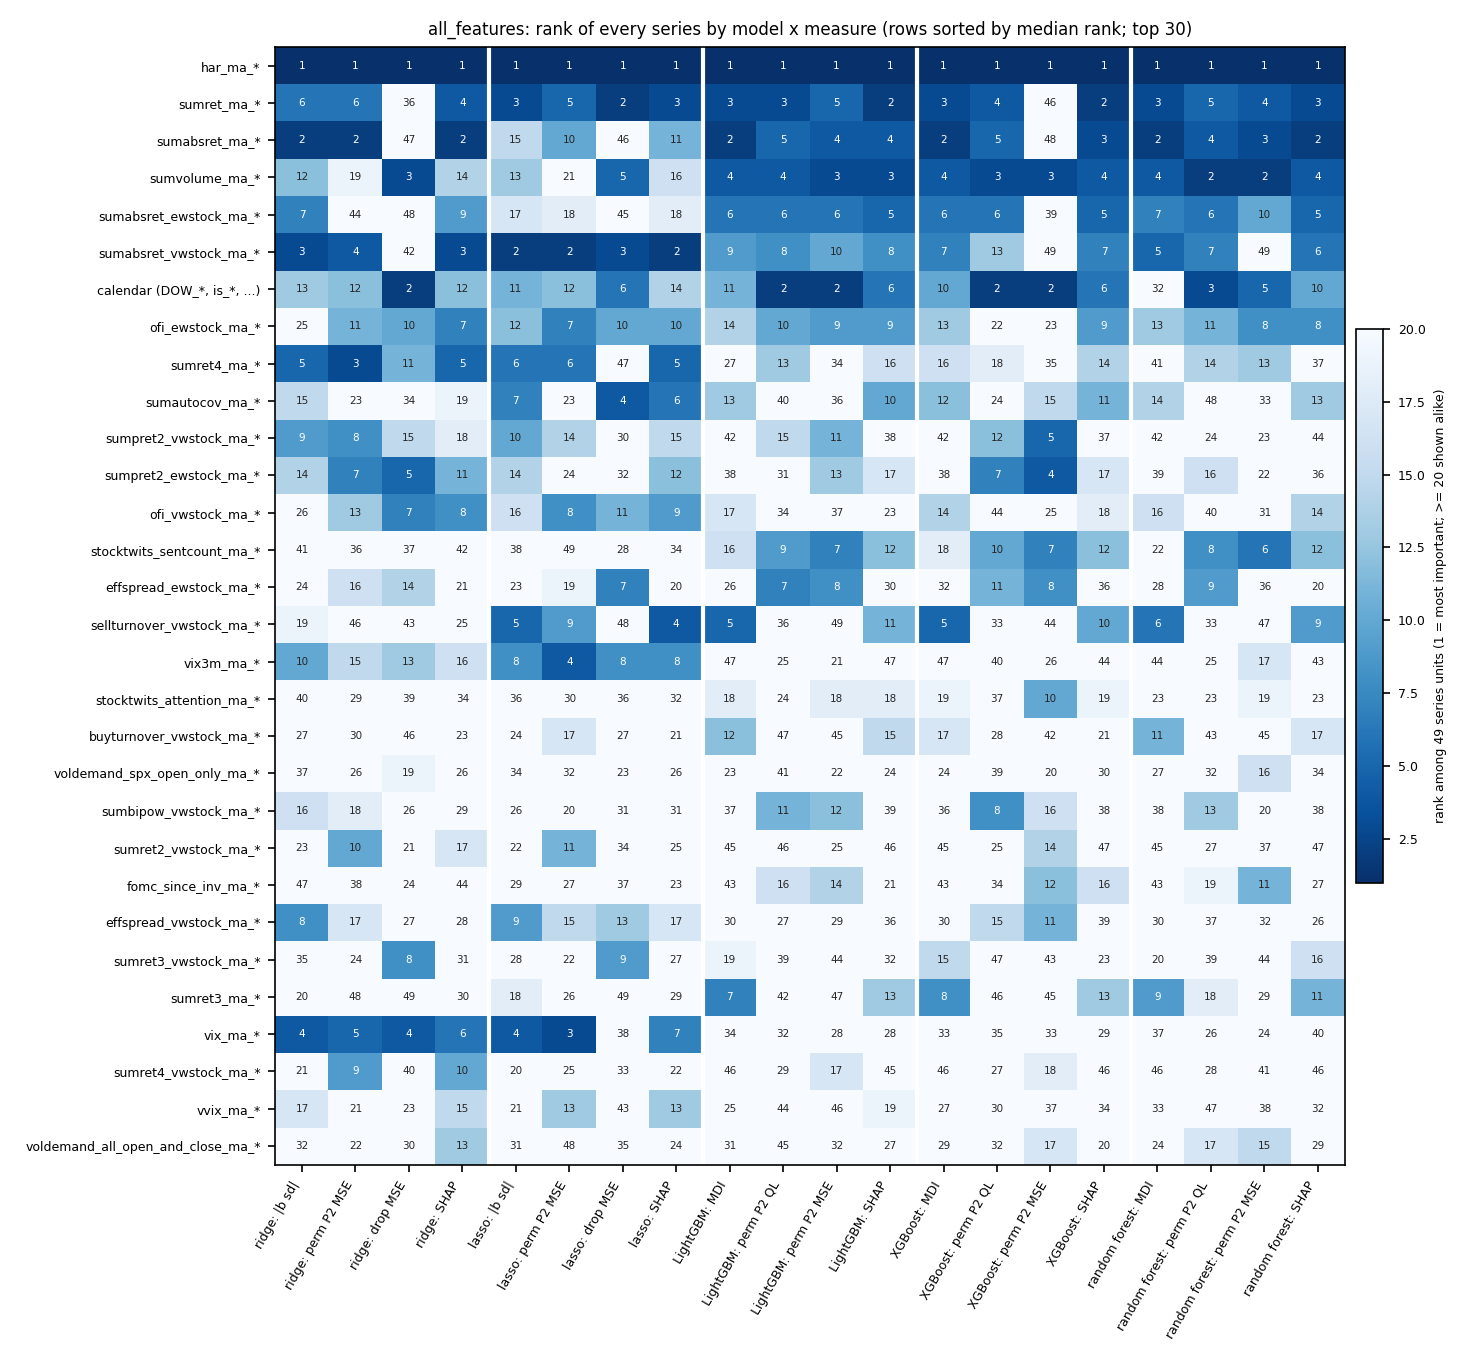
\includegraphics[width=\linewidth]{../results/feature_importance_1530_dedup/fig_rank_heatmap_all_features_series.png}
% % 2026-10-15 (notation pass): parked -- code jargon (all features, |beta . sd|, P2); American spelling
% % \caption{Draft, measures under review. The rank of each series among the \rhappFiSeries{} by model $\times$ measure,
% % all features (1 = most important; the colour scale saturates, so the low ranks share a shade); rows sorted by median rank,
% % the leading rows shown. Measures: $|\beta\cdot\mathrm{sd}|$ and drop-column $\Delta$MSE (linear), MDI\,/\,gain
% % (trees), permutation P2 on QLIKE (QL) or MSE, and SHAP.}
% \caption{Draft, measures under review. Rank of each predictor series among the \rhappFiSeries{}, by model and
% importance measure, closing-interval models on the full predictor set (1 = most important; the color scale saturates,
% so low ranks share a shade). Rows are sorted by median rank; the leading rows are shown. Measures:
% $|\beta_j|\,\mathrm{sd}(x_j)$ and the drop-column increase in squared-error loss (linear models), MDI or gain (trees),
% permutation importance on QLIKE (QL) or on squared-error loss (MSE), and SHAP.}
% \label{fig:rh_app_fi_heat_series}
% \end{figure}

% Source: results/feature_importance_1530_dedup/fig_rank_heatmap_all_features_cluster.png (raster)
% 2026-10-15 (user): parked -- non-standard figure; focus on legible tables
% \begin{figure}[htbp]
% \centering
% 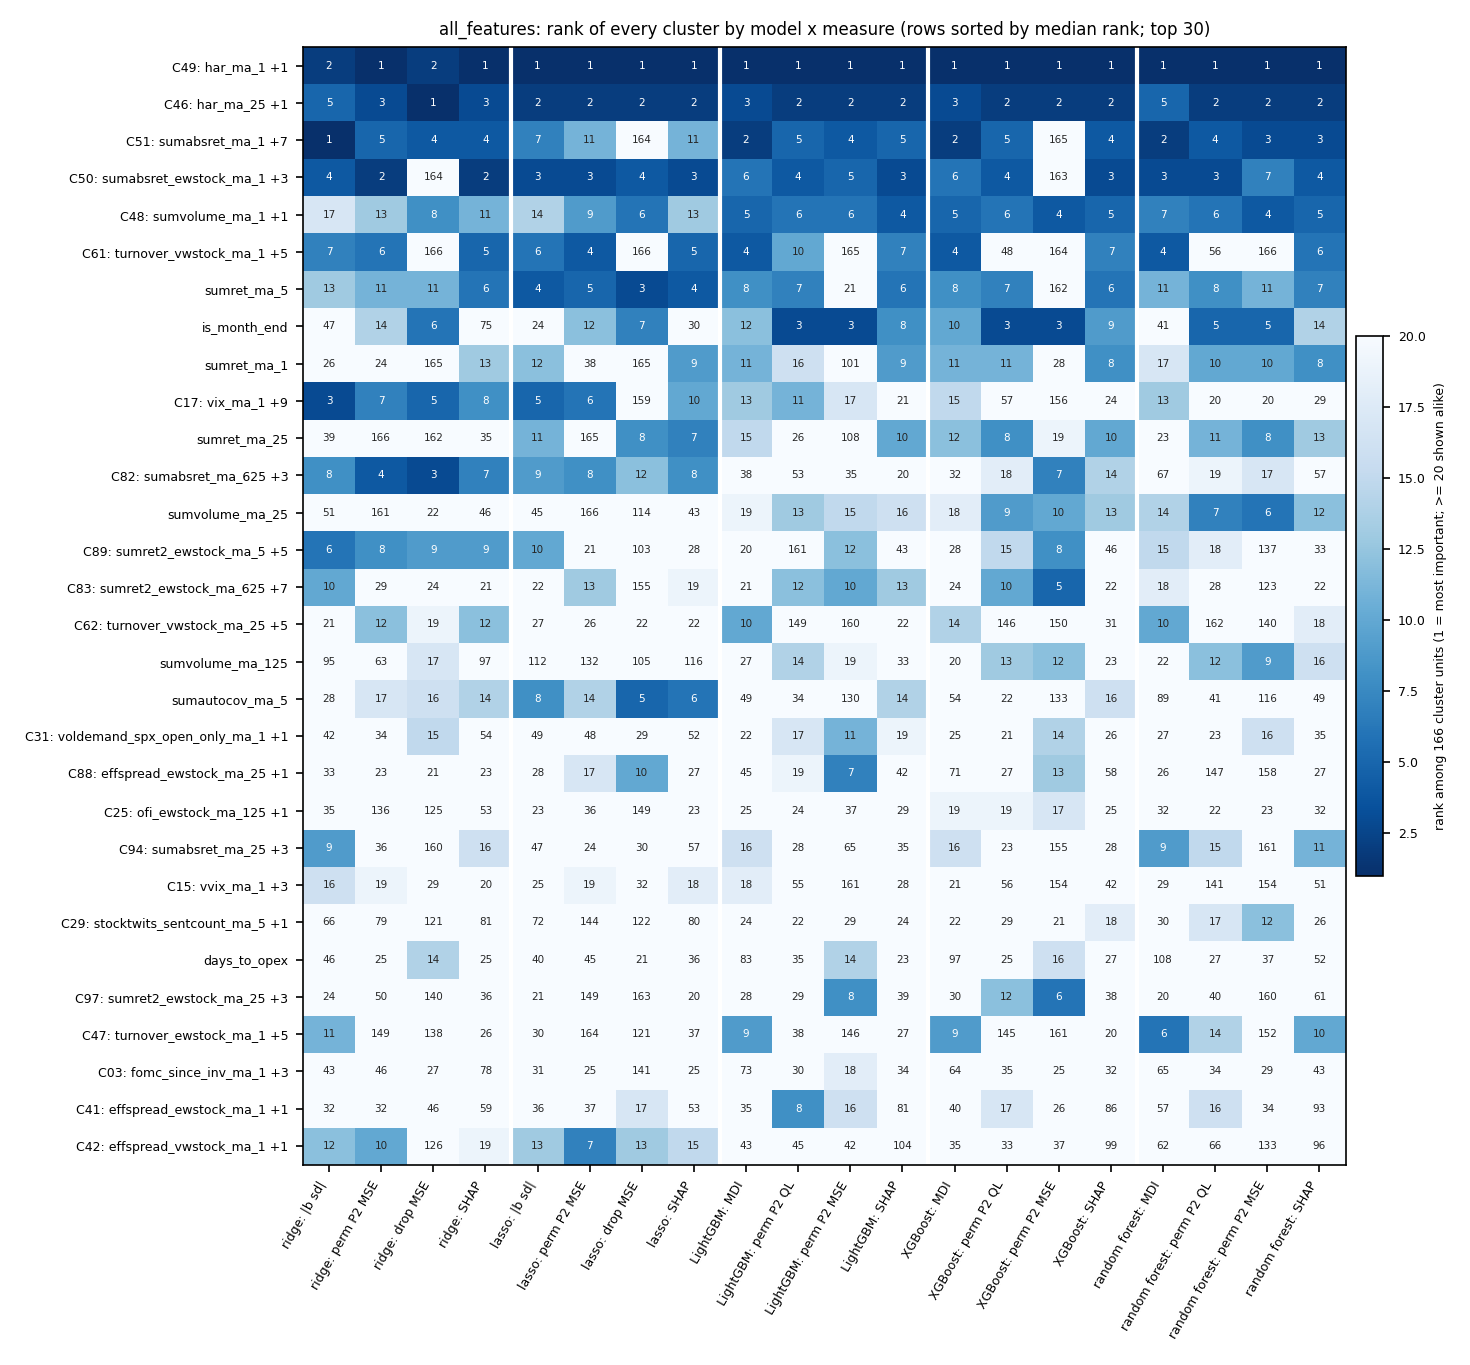
\includegraphics[width=\linewidth]{../results/feature_importance_1530_dedup/fig_rank_heatmap_all_features_cluster.png}
% % 2026-10-15 (notation pass): parked -- wording; explicit cross-reference
% % \caption{Draft, measures under review. The same at the cluster level: \rhappFiClusters{} clusters of columns, every
% % pair in a cluster correlated at $|\rho| \ge \rhappFiClusterCorr$ (complete linkage). A cluster is named by its first
% % member and the number of further members ($+k$); single columns keep their name.}
% \caption{Draft, measures under review. As Figure~\ref{fig:rh_app_fi_heat_series}, at the cluster level:
% \rhappFiClusters{} clusters of columns, formed by complete-linkage clustering so that every pair of columns within a
% cluster has absolute correlation $|\rho| \ge \rhappFiClusterCorr$. A cluster is labeled by its first member and the
% number of further members ($+k$); singleton columns keep their own label.}
% \label{fig:rh_app_fi_heat_cluster}
% \end{figure}

% Source: figures/feature_importance_1530_over_time.pdf (vector)
% 2026-10-15 (user): parked -- non-standard figure; focus on legible tables
% \begin{figure}[htbp]
% \centering
% 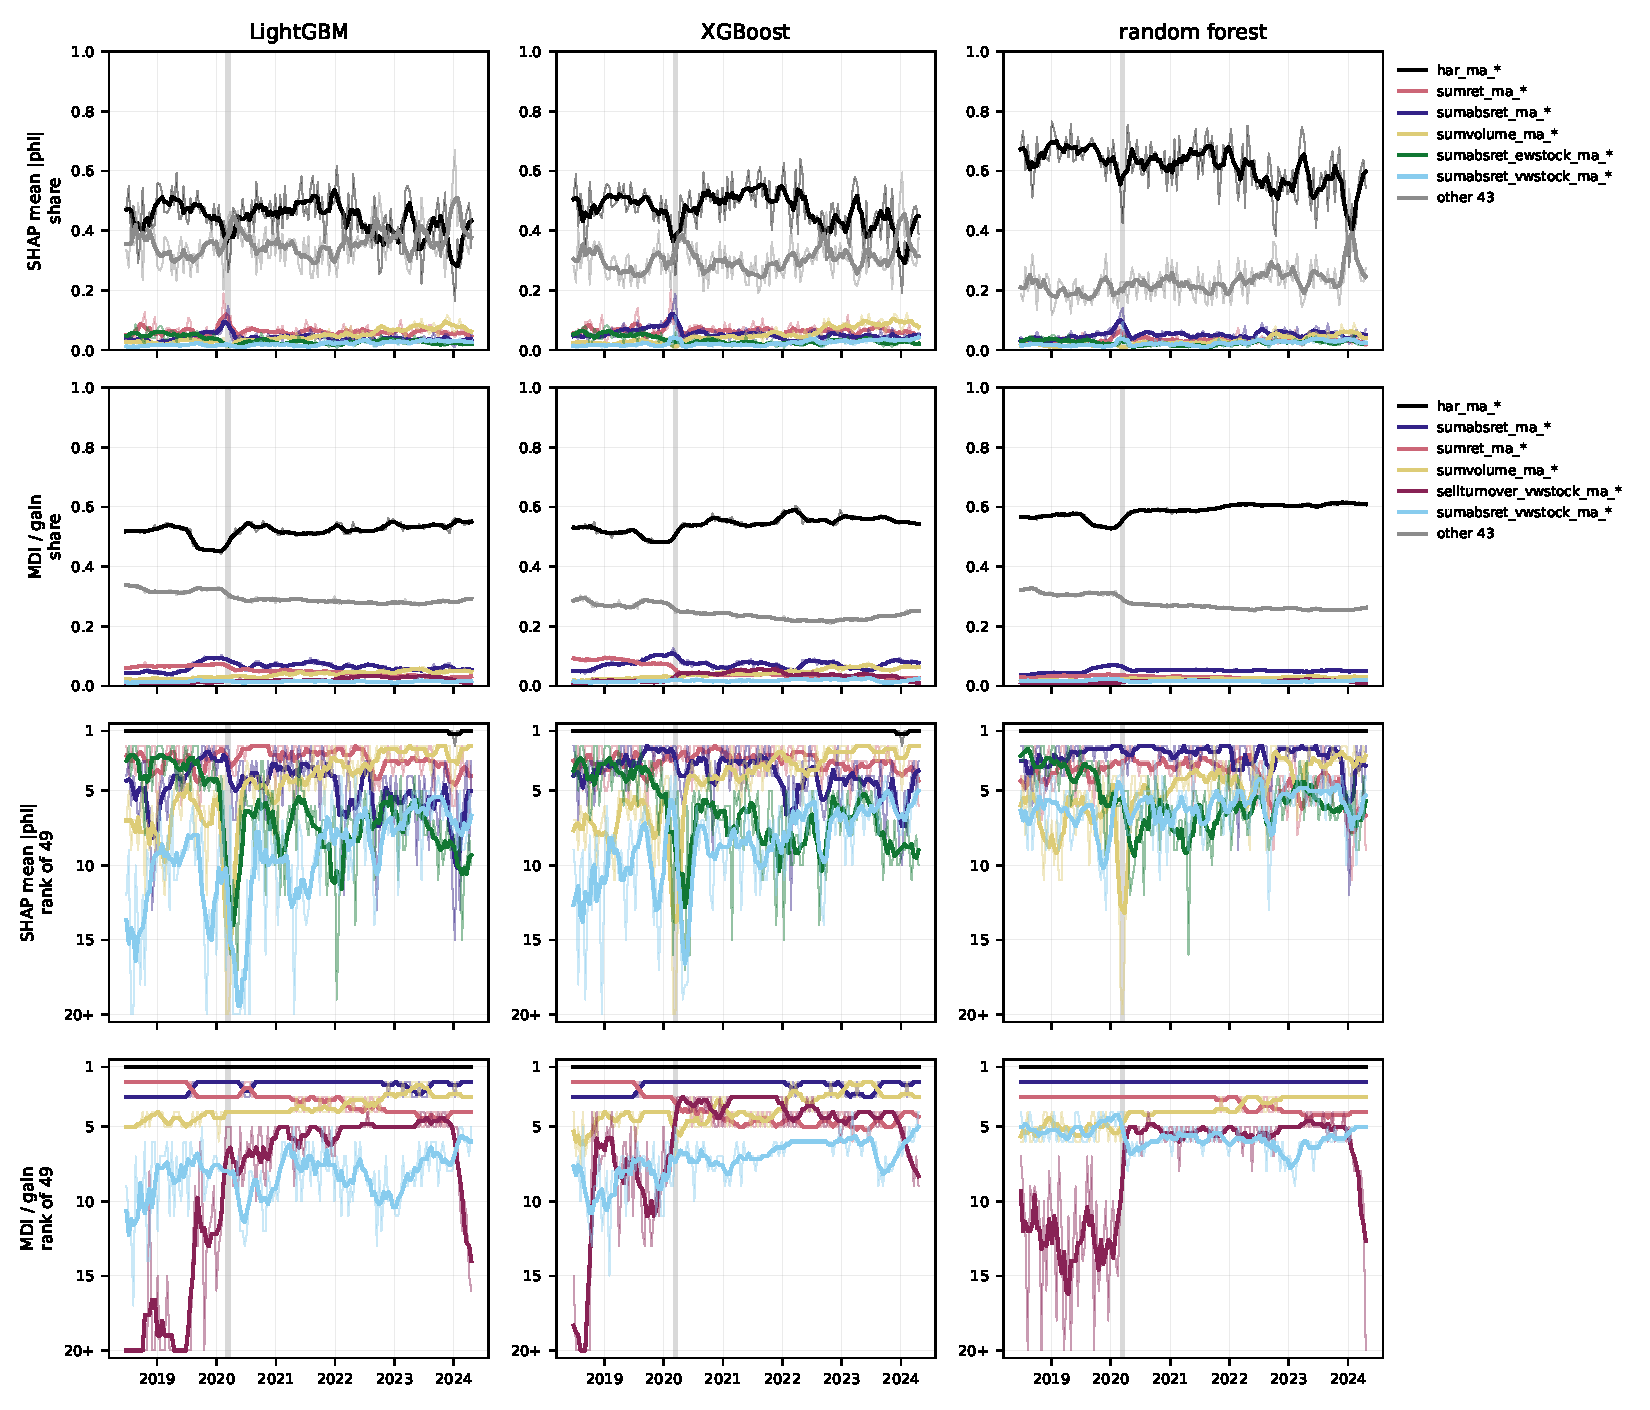
\includegraphics[width=\linewidth]{figures/feature_importance_1530_over_time.pdf}
% % 2026-10-15 (notation pass): parked -- code jargon (refit, held-out tail, har_ma_*, sessions); American spelling
% % \caption{Draft, measures under review. Importance over time, the three trees, all features, series level. Rows 1--2:
% % each series' share of the refit's total SHAP mean $|\phi|$ (on the held-out tail) and MDI\,/\,gain; rows 3--4: the
% % same series' rank among the \rhappFiSeries{} (ranks beyond \rhappFiTimeCap{} drawn at \rhappFiTimeCap). Lines:
% % \texttt{har\_ma\_*} and the next \rhappFiTimeTop{} series by overall share, the rest summed as `other'. Thin: one
% % point per refit (every \rhappFiRefitEvery{} sessions, \rhappFiRefits{} refits), at its tail's start date; thick: a
% % \rhappFiTimeSmooth-refit centred rolling mean. Grey band: the 2020 crash tails. Shares are split credit: correlated
% % inputs share it, and MDI and SHAP favour many-valued columns.}
% \caption{Draft, measures under review. Predictor importance over time for the three closing-interval tree models on
% the full predictor set, at the series level. Rows 1--2: each series' share of the re-estimation's total mean absolute
% SHAP value (on its out-of-sample block) and of its total MDI or gain; rows 3--4: the same series' rank among the
% \rhappFiSeries{} (ranks beyond \rhappFiTimeCap{} drawn at \rhappFiTimeCap). Lines: the HAR components
% $\bar y^{(k)}_t$ and the next \rhappFiTimeTop{} series by overall share, with the remainder summed as `other'. Thin
% lines: one point per re-estimation (every \rhappFiRefitEvery{} trading days, \rhappFiRefits{} re-estimations), dated
% at the start of its out-of-sample block, i.e., the trading days it forecasts before the next re-estimation; thick
% lines: a centered rolling mean over \rhappFiTimeSmooth{} re-estimations. Gray band: out-of-sample blocks in the 2020
% crash. Shares split credit: correlated predictors share it, and MDI and SHAP favor columns with many distinct
% values.}
% \label{fig:rh_app_fi_time_trees}
% \end{figure}

% Source: figures/feature_importance_1530_over_time_linear.pdf (vector)
% 2026-10-15 (user): parked -- non-standard figure; focus on legible tables
% \begin{figure}[htbp]
% \centering
% 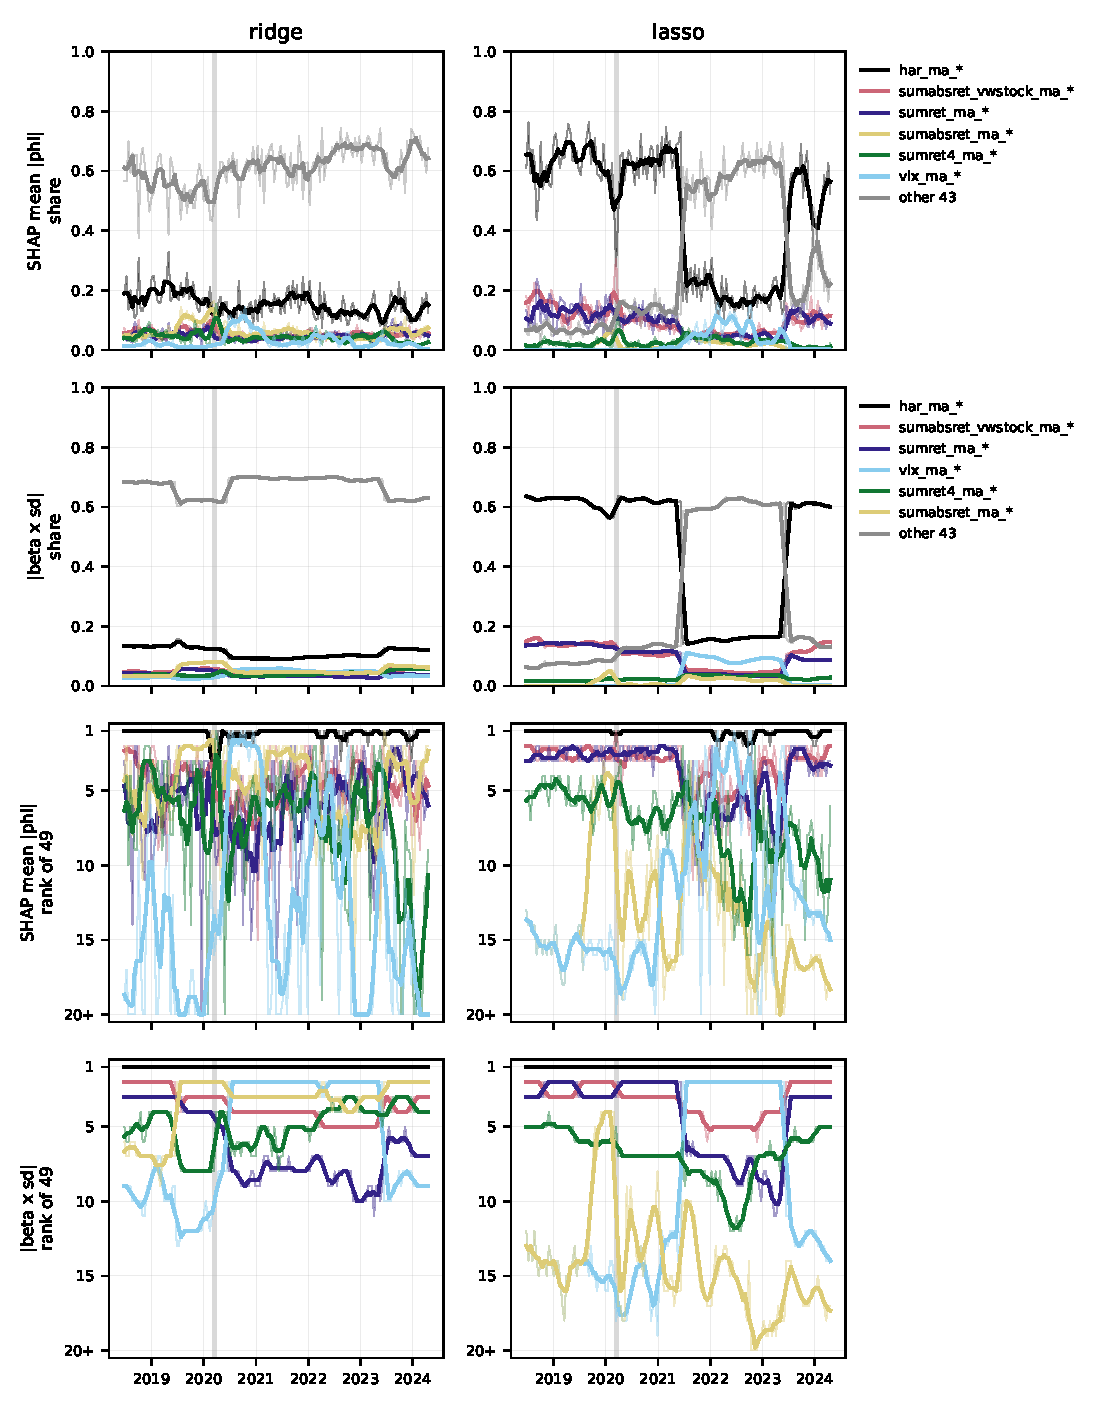
\includegraphics[width=\linewidth,height=0.78\textheight,keepaspectratio]{figures/feature_importance_1530_over_time_linear.pdf}
% % 2026-10-15 (notation pass): parked -- code jargon (per-bar, refit's window, |beta . sd|); explicit cross-reference
% % \caption{Draft, measures under review. The same for the per-bar ridge and lasso: SHAP mean $|\phi|$, with
% % $\phi_{t,j} = \beta_j(x_{t,j} - \bar x_j)$ and the window mean as background, and $|\beta\cdot\mathrm{sd}|$ (the
% % coefficient times the column's standard deviation in the refit's window, summed over a series' columns), as shares
% % and as ranks. A linear model spreads or concentrates credit across correlated columns differently from a tree, so
% % the shares compare over time within a model, not across the two figures.}
% \caption{Draft, measures under review. As Figure~\ref{fig:rh_app_fi_time_trees}, for the closing-interval ridge and
% lasso: the mean absolute SHAP value, with $\phi_{t,j} = \beta_j(x_{t,j} - \bar x_j)$ and the estimation-window mean
% $\bar x_j$ as background, and $|\beta_j|\,\mathrm{sd}(x_j)$, the absolute coefficient times the column's standard
% deviation in the estimation window, summed over a series' columns; both as shares and as ranks. A linear model
% spreads or concentrates credit across correlated columns differently from a tree, so the shares are comparable over
% time within a model, not across the two figures.}
% \label{fig:rh_app_fi_time_linear}
% \end{figure}

% Source: generated/appendix_campaign_16h_featimp.tex (re-laid out: generated/rehaul_app_featimp_harma.tex)
\begin{table}[htbp]
\centering
\small
\begin{threeparttable}
% 2026-10-15 (notation pass): parked -- code identifier har_ma_* and 'ladder' replaced by 'HAR components'
% \caption{Draft, measures under review. The \texttt{har\_ma\_*} ladder's importance in the trees, first pass to
% the current design (all features), old $\to$ new.}
% 2026-10-15 (table legibility): short caption, details in the notes; notes cut to about five sentences, method
% details referred to Methods. The pre-notation-pass caption and notes are parked in the comments here.
\caption{Importance of the HAR components in the tree models}
\label{tab:rh_app_fi_harma}
% AUTO-GENERATED by writeup/make_rehaul_appendix.py -- do not edit.
% Source: writeup/generated/appendix_campaign_16h_featimp.tex (numbers verbatim; its sources are listed there)
\begin{tabular}{@{}l*{5}{c}@{}}
\toprule
 & MDI & SHAP & Permutation & Close-interaction & MDI \\
Model & share (\%) & share (\%) & $\Delta$QLIKE (\%) & share (\%) & rank \\
\midrule
LightGBM & $57 \to 52$ & $47 \to 44$ & $237 \to 200$ & $22$ & $1 \to 1$ \\
XGBoost & $69 \to 54$ & $55 \to 47$ & $224 \to 181$ & $22$ & $1 \to 1$ \\
Random forest & $62 \to 59$ & $58 \to 61$ & $290 \to 271$ & $54$ & $1 \to 1$ \\
\bottomrule
\end{tabular}

\begin{tablenotes}[flushleft]
\footnotesize
% 2026-10-15 (notation pass): parked -- code jargon (ladder, unmasked, window-masked, P2, tail loss, _x_close)
% \item[] \emph{Notes:} first pass: the old design (with the \rhappNsessionEdge{} session-edge interactions), trees
% unmasked; new: those columns dropped and every tree fit window-masked. MDI and TreeSHAP: the ladder's share of the
% model's total. Perm.\ P2 $\Delta$QLIKE: the loss increase when the ladder's rows are replaced by rows drawn from the
% training window, in \% of the model's tail loss. \texttt{\_x\_close} share: the part of the old ladder's MDI that sat
% on its \rhappNsessionEdgeHalf{} \texttt{\_x\_close} copies. MDI rank among the series. XGBoost and the random forest
% also changed settings between the passes, so their before/after mixes that change with the design and the mask.
\item[] \textit{Notes:} Draft, measures under review. Closing-interval tree models on the full predictor set, first
pass (old) $\to$ current design (new); the first pass includes the \rhappNsessionEdge{} interactions of the HAR
components with the opening- and closing-session dummies and no column screening, the current design drops those
interactions and screens out constant and duplicate columns in every estimation window. MDI and TreeSHAP: the HAR
components' share of the model's total; permutation $\Delta$QLIKE: the increase in QLIKE when their values are
replaced by rows drawn from the estimation window, in percent of the model's out-of-sample loss. Close-interaction
share: the part of the old MDI carried by the \rhappNsessionEdgeHalf{} closing-session interactions, which at the
closing interval are copies of the HAR components; MDI rank: rank among the series. XGBoost and the random forest
also changed hyperparameters between the passes, so their changes mix design, screening and hyperparameters.
\end{tablenotes}
\end{threeparttable}
\end{table}
